% !TEX program = xelatex
\documentclass[final]{beamer}

\usepackage{iftex}
\ifPDFTeX
  \usepackage[T1]{fontenc}         % pdfLaTeX only
\fi
\ifLuaTeX
  \usepackage[utf8]{luainputenc}
\fi
\usepackage{lmodern}
% True A1 landscape (841 x 594 mm) so the poster fits A1 paper exactly.
\usepackage[size=a1,orientation=landscape,scale=0.9]{beamerposter}
\usetheme{gemini}
\usecolortheme{msu}
\usepackage{graphicx}
\usepackage{caption}
\usepackage{booktabs}
\usepackage{amsmath,amssymb}
\usepackage{tikz}
\usepackage{pgfplots}
\usepackage{multicol}
\usepackage{anyfontsize}
\usepackage{qrcode}
\usepackage{url}

\usetikzlibrary{arrows.meta, positioning, shapes.geometric, calc}
\pgfplotsset{compat=1.18}

% Figures live with the report; reference them by bare filename.
\graphicspath{{../report/images/}{./}}

\newlength{\sepwidth}
\newlength{\colwidth}
\setlength{\sepwidth}{0.025\paperwidth}
\setlength{\colwidth}{0.3\paperwidth}
\newcommand{\separatorcolumn}{\begin{column}{\sepwidth}\end{column}}
% Report not finished yet — QR target is a placeholder until the link exists.
\newcommand{\reporturl}{TOBEDONE}
\setbeamerfont{headline title}{size=\Large, series=\bfseries}

% ── Placeholder boxes for not-yet-finished content ──────────────────────────
% Heights are chosen to match the real fragment they will be replaced by.
\newcommand{\todobox}[2]{%
  \begin{center}
  \begin{tikzpicture}
    \node[draw=orange!85!black, dashed, line width=1.3pt, rounded corners=16pt,
          fill=orange!9, text=orange!55!black, font=\itshape\bfseries,
          align=center, inner sep=11pt,
          text width=\dimexpr\linewidth-34pt\relax, minimum height=#1]
      {#2};
  \end{tikzpicture}
  \end{center}}
% Width-matched variant: \todoboxw{<width>}{<height>}{<text>}
\newcommand{\todoboxw}[3]{%
  \begin{center}
  \begin{tikzpicture}
    \node[draw=orange!85!black, dashed, line width=1.3pt, rounded corners=16pt,
          fill=orange!9, text=orange!55!black, font=\itshape\bfseries,
          align=center, inner sep=11pt,
          text width=\dimexpr#1-34pt\relax, minimum height=#2]
      {#3};
  \end{tikzpicture}
  \end{center}}

\title{Investigating the Impact of REPA Loss on Training Speed and Generation Quality in Diffusion Models}
\author{Evgenii Pakhomov, Dmitrii Gromak, Sergei Kopylov, Miron Makhlin, Vladimir Novikov}
\institute[HSE]{HSE University, Methods of Optimization in Machine Learning course}

\footercontent{\hfill MOML course project \hfill}
\logoright{
\includegraphics[height=4.8cm]{hse_logo.pdf}}

\begin{document}
\begin{frame}[t]
\small
\begin{columns}[t]
\separatorcolumn

%==================== COLUMN 1 — Problem, Method, Theory, Toy model ====================
\begin{column}{\colwidth}

\begin{block}{Motivation}
\textbf{REPA} accelerates diffusion training by aligning a transformer's hidden states with clean features from a
frozen encoder (DINOv2). We ask \emph{when} this helps, show that a constant alignment weight eventually hurts and
compare effects on different single-domain datasets.
\end{block}

\begin{block}{The Problem: Gradient Conflict}
We track the cosine between the diffusion and REPA gradients,
$c = \cos\!\big(\nabla_w \mathcal{L}_{\mathrm{diff}},\ \nabla_w \mathcal{L}_{\mathrm{REPA}}\big)$.
It is \emph{positive} at high noise but turns \emph{negative} at low noise and late in training -- there the
auxiliary term pulls the update \emph{against} the diffusion objective.
\begin{figure}
  \centering
  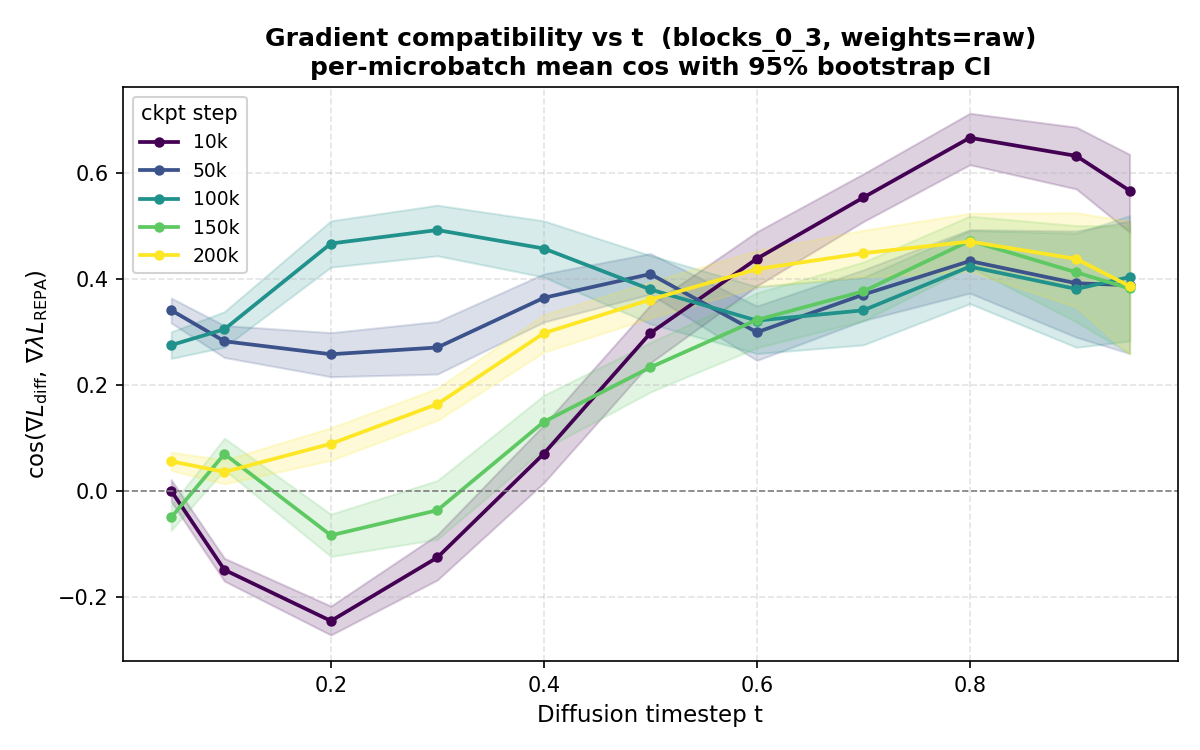
\includegraphics[width=0.72\linewidth]{1_cos_vs_t__blocks_0_3__raw.png}
  \caption{$c$ vs.\ timestep $t$ (high $t=$ high noise). Note the negative region at low $t$.}
\end{figure}
\end{block}

\begin{block}{REPA-$\Sigma$: Method \& Guarantees}
Discard \emph{only} the part of the REPA gradient $r$ anti-aligned with an EMA estimate $\bar g$ of the diffusion
gradient $g$:
\[ r^{\Sigma}=r-\frac{[\langle r,\bar g\rangle]_-}{\|\bar g\|_2^2}\,\bar g,\qquad [x]_-=\min(x,0). \]
\textbf{Minimal change:} projection of $r$ onto $\{r':\langle r',\bar g\rangle\ge0\}$.\\
\textbf{Non-interference:} $\langle g+\lambda r^{\Sigma},\bar g\rangle\ge\langle g,\bar g\rangle$ for all
$\lambda\ge0$ -- the adapted gradient never works against the diffusion descent direction.
\end{block}

\begin{block}{Toy Model: Whitened Linear Setting}
\textbf{Setting.} Let $x_0\in\mathbb R^d$ be a clean sample. We assume whitened features $u$ with $\mathbb E[uu^\top]=I$ and a
linear denoiser $\hat x_0=Bu$. The diffusion loss $L_{\mathrm{diff}}(B)=\tfrac12\mathbb E\|Bu-x_0\|^2$ has the unique optimum
$A=\mathbb E[x_0u^\top]$. We consider a teacher which projects onto an $r$-dim semantic subspace ($P^2=P$, $Q=I-P$), giving
$L_{\mathrm{repa}}(B)=\tfrac12\mathbb E\|Bu-Px_0\|^2$ -- it keeps the semantic part $Px_0$ and \emph{drops} the detail $Qx_0$.

\textbf{Result.} Standard REPA minimises $L_{\mathrm{diff}}+\lambda L_{\mathrm{repa}}$, with optimum
$B^\star_\lambda = PA + \tfrac{1}{1+\lambda}\,QA$: the detail is shrunk, so it \emph{cannot} reach $A$ for
$\lambda>0$. REPA-$\Sigma$ keeps $A$ a stationary point for every $\lambda$ -- it provably reaches the optimal
denoiser $A$ while still using the alignment signal (under some extra assumptions).
\end{block}

\begin{block}{Toy Experiments}
Experiments supporting the Toy Model results above -- empirically confirming that REPA-$\Sigma$ reaches the
optimal denoiser $A$ while vanilla REPA stays biased.
\todobox{5.2cm}{\normalfont\upshape
(1) Diagonal-matrix model with an independent-features teacher -- closed-form convergence to $A$ under
REPA-$\Sigma$ vs.\ biased REPA. \quad
(2) MLP denoiser on MNIST/CIFAR trained with a REPA-style teacher matching our setting.}
\end{block}

\end{column}

\separatorcolumn

%==================== COLUMN 2 — Convergence (3 datasets, equal size) ====================
\begin{column}{\colwidth}

\begin{block}{Convergence across Three Datasets}
This section compares the impact of REPA vs.\ REPA-$\Sigma$ (w or w/o $\lambda$-anneal), against the
diffusion baseline, on convergence speed (FID) across three single-domain datasets spanning a
spatial-difficulty axis (the lower the dataset, the harder it is).

We plan to compare convergence curves between datasets.

On \textbf{CelebA}, surgery helps mid-training and $\lambda$-annealing late; combining
both gives the best final FID.
\begin{figure}
  \centering
  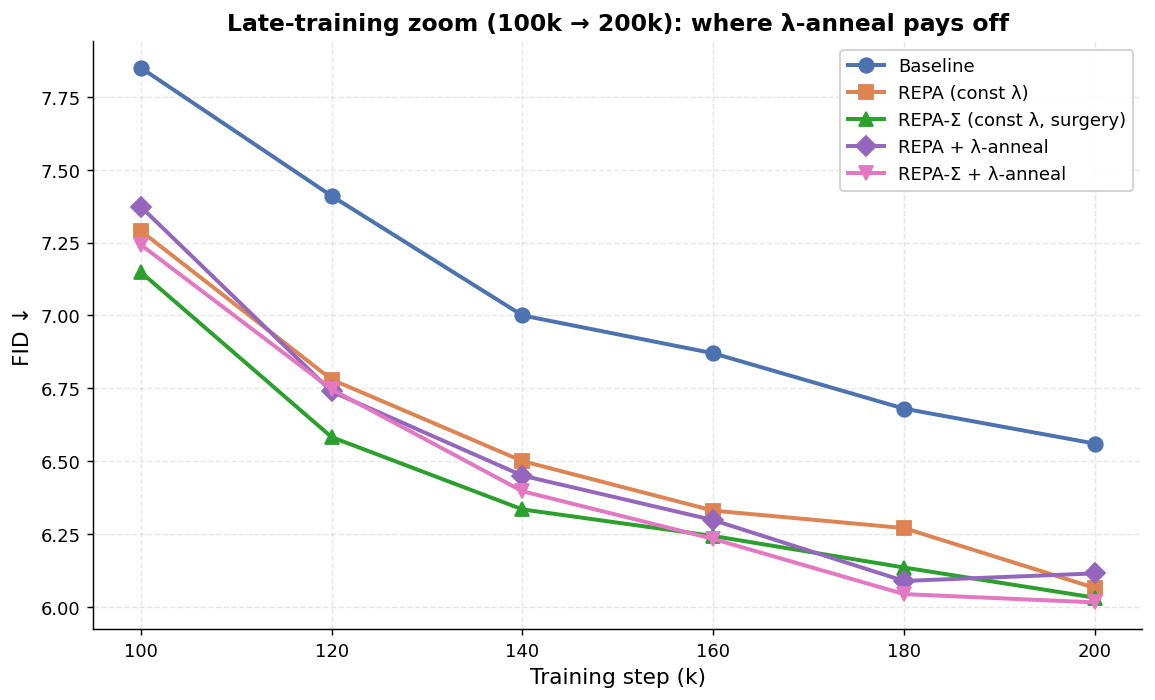
\includegraphics[width=\linewidth]{fid_100k_200k.png}
  \caption{CelebA -- late-training FID. REPA-$\Sigma$ $+\,\lambda$-anneal wins.}
\end{figure}
\vspace{0.2em}
\todobox{12.6cm}{LSUN Church \\[0.3em]\normalfont\upshape FID/KID convergence: baseline vs.\ REPA vs.\
REPA-$\Sigma$ ($\pm\,\lambda$-anneal), plus the gradient-compatibility curve.}
\vspace{0.6em}
\todobox{12.6cm}{Comprehensive Cars (CompCars) \\[0.3em]\normalfont\upshape Same convergence comparison
across all methods.}
\end{block}

\end{column}

\separatorcolumn

%==================== COLUMN 3 — Feature maps (3 datasets, equal size) + report ====================
\begin{column}{\colwidth}

\begin{block}{Feature Maps \& Generation across Three Datasets}
This section compares the impact of REPA vs.\ REPA-$\Sigma$ using PCA feature maps and
generations across the three datasets. In CelebA PCA maps show REPA preserves semantic, face-centred structure through the
mid-network and under heavy noise, where the baseline collapses; we extend the comparison to all three domains.

We plan to compare feature maps between datasets.

\begin{figure}
  \centering
  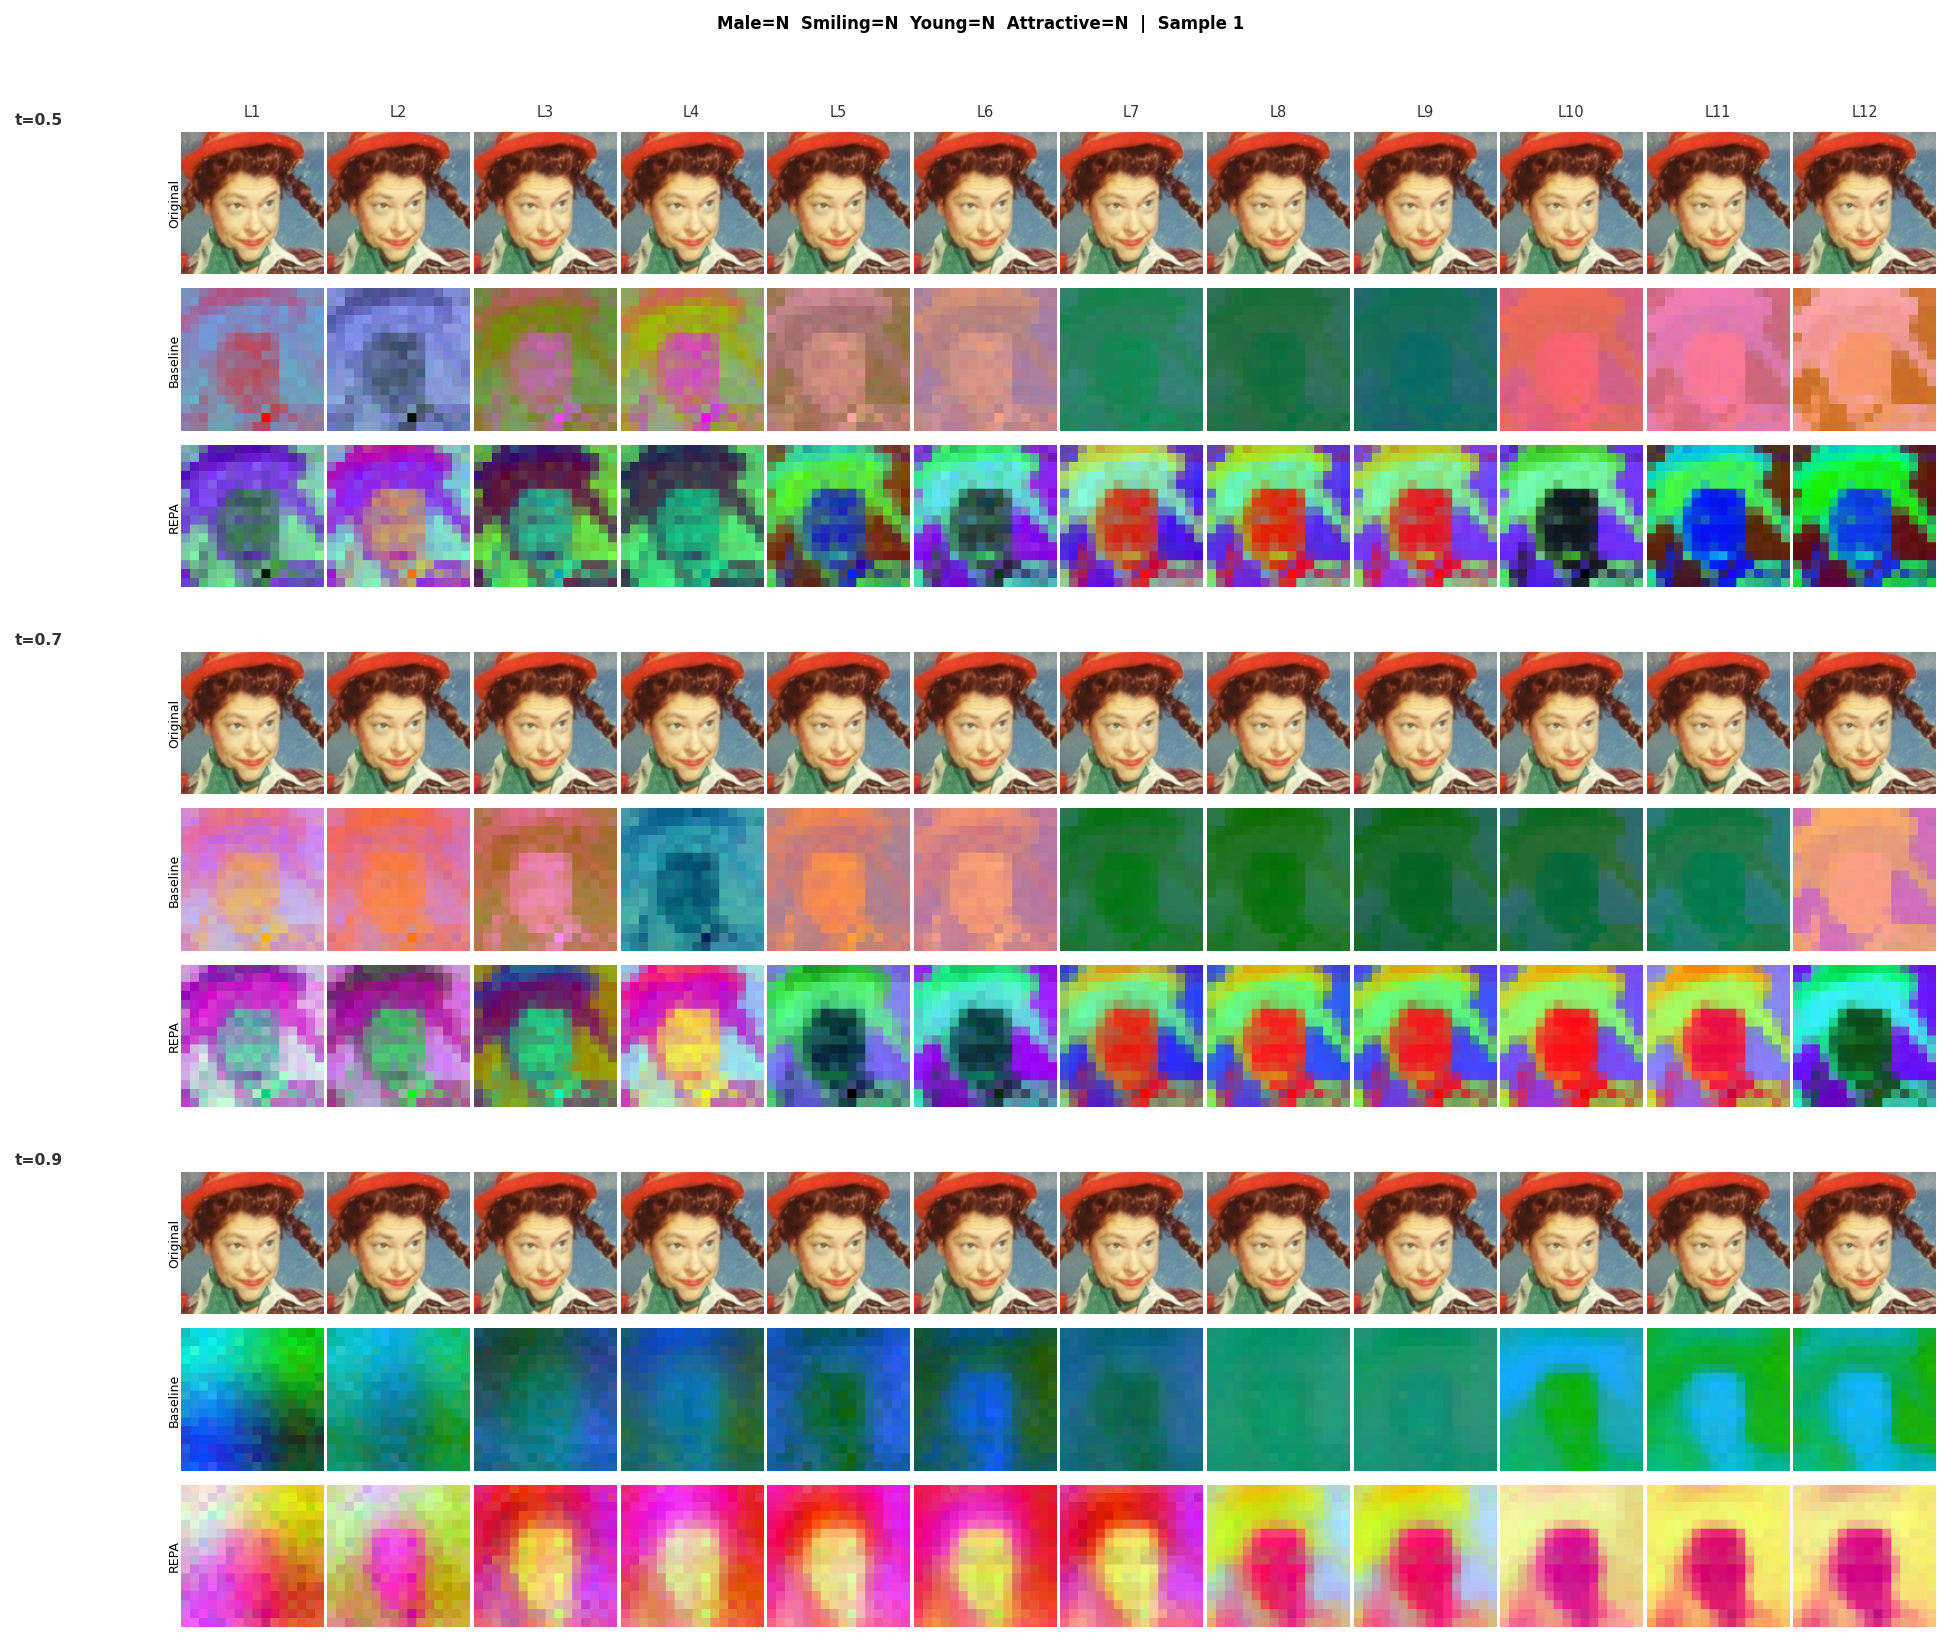
\includegraphics[width=0.62\linewidth]{noise_layers.png}
  \caption{CelebA -- per-block PCA maps: image / Baseline / REPA.}
\end{figure}
\vspace{0.1em}
\todoboxw{0.62\linewidth}{10.8cm}{LSUN Church \\[0.3em]\normalfont\upshape PCA feature maps \& generation samples
(baseline / REPA / REPA-$\Sigma$).}
\vspace{0.5em}
\todoboxw{0.62\linewidth}{10.8cm}{Comprehensive Cars \\[0.3em]\normalfont\upshape PCA feature maps \&
generation samples.}
\end{block}

\begin{alertblock}{Full Report}
\begin{center}
  \qrcode[height=1.5in]{\reporturl}\\[0.4ex]
  {\small Full report -- link to be added}
\end{center}
\end{alertblock}

\end{column}

\separatorcolumn
\end{columns}
\end{frame}
\end{document}
